\documentclass{school-22.211-notes}
\date{March  5, 2012}

\begin{document}
\maketitle


%%%%%%%%%%%%%%%%%%%%%%%%% Resonance Models Day 5 %%%%%%%%%%%%%%%%%%%%%%%%%%%%
\lecture{Finite Medium Spatial Self-Shielding: Two Region Approximations} \label{heterogeneous-geo}
This is probably the most important topic in generating cross section in reactor physics. We want to take into account both the spatial and energy structure distributions of flux within each resonance when solving the neutron slowing down problem. 

Historically we have learnt early on that we need to lump resonant materials together to get criticality, which leads to the understanding of spatial self-shielding. More specifically, we want to produce accurate multi-group cross sections, for which the energy group width is very broad compared to any single resonance. All details of the spatial and energy structure distribution of flux within each resonance must be treated when solving the neutron slowing down problem. 
\begin{enumerate}
\item Assumptions for heterogeneous geometry resonant approximations:
\begin{itemize}
\item Moderator are purely scattering;
\item Moderator scattering xs is independent of energy;
\item The previous two points together leads to that the slowing down energy source in fuel and moderator is 1/E;
\item Slowing down source is spatially uniform within each region. This is the case for non-resonant energy; and we can make this assumption for resonant energies is because there is no much scattering in at a resonant energy. \textit{This is the only additional assumption we are making compare with the previous section}
\item A single resonance absorber species exists only in the fuel;
\item Fuel scattering removes neutrons from resonance energy (that is, narrow resonance model); 
\end{itemize}

\item Spatial Reciprocity Theorem. First we introduce the reciprocity condition. The only assumption we make for this theorem is that the source is flat. This theorem does not depend on geometry. 

Given two homogeneous region 1 and 2, the probability of going from point A in 1 to point B in 2 without colliding is:
\eqn{ \frac{e^{-\tau}}{4 \pi R^2} }
where $\tau = \frac{x_1}{\lambda_1} + \frac{x_2}{\lambda_2} = x_1 \Sigma_1 + x_2 \Sigma_2$. The probability of going from A to B and then colliding at B is: 
\eqn{ \frac{e^{-\tau}}{4 \pi R^2} \Sigma_2 }
The probability of going from A to any point in region 2 and colliding is:
\eqn{ \int \frac{e^{-\tau}}{4 \pi R^2} \Sigma_2  \dV_2}
The probability of a uniform spatial neutron source in region 1 going to any point in region 2 and colliding is:
\eqn{ \int \dV_1 \int \frac{e^{-\tau}}{4 \pi R^2} \Sigma_2  \dV_2}
\hi{First flight probability $P_{ij}$} describes the probability that a neutron born in $V_i$ will make its first collision in $V_j$ (the average probability per unit volume of a uniform source neutron going from region 1 to 2 and colliding):
\eqn{ P_{1\to 2} = \frac{\Sigma_2}{V_1} \int \dV_1 \int \frac{e^{-\tau}}{4 \pi R^2}  \dV_2}
Likewise,
\eqn{ P_{2\to 1} = \frac{\Sigma_1}{V_2} \int \dV_2 \int \frac{e^{-\tau}}{4 \pi R^2}  \dV_1}
Since the two integrals are symmetric (that is, $P_{A\to B}$ and $P_{B \to A}$ are essentially the same), we can write,
\eqn{ P_{1\to 2} \frac{V_1}{\Sigma_2} = P_{2\to 1} \frac{V_2}{\Sigma_1} }
Hence we reach the reciprocity condition:
\eqn{ \boxed{ P_{1\to 2} \Sigma_1 V_1 = P_{2\to 1} \Sigma_2 V_2 } }
\hi{This is entirely general in geometry so far} (maybe require convex geometry?) as we are just saying that the attenuation coefficient is the same forward and backward. 


\item Two Region Balance Equations. 
First collision reaction rate balance, where $\sigma_{t,f}(u) = \sigma_{r,f} + \sigma_{pot, f}$ (the resonance absorption xs plus the potential scattering xs):
\eqn{ \overbrace{N_f \sigma_{t,f} (u) \Phi(u) V_f}^{\mbox{fuel region lost neutrons}} = \overbrace{Q_f V_f P_{f\to f} + Q_m V_m P_{m\to f}}^{\mbox{fuel region gain neutrons from slowing down sources}}  }
Because slowing down sources in both fuel and moderator are assumed to arise from the 1/E flux above the resonance energy, we can write
\eqn{ Q_m &= N_m \sigma_{s,m} \Psi(u) &  Q_f&= N_f \sigma_{pot, f} \Psi(u) }
Plug the slowing down sources back into the reaction rate balance equation, and recall $\Phi(u) = \Psi(u) \phi(u)$ where $\phi(u)$ is the fine structure energy shape of the flux for homogeneous mixture, we extand the definition to define $\phi_f(u)$ as the heterogeneous energy shape of flux in fuel,
\eqn{ N_f \sigma_{t,f} (u) \phi_f (u) V_f = N_f \sigma_{pot, f} V_f P_{f\to f} + N_m \sigma{s,m} V_m P_{m\to f} }
Next we use reciprocity relationship,
\eqn{ P_{m\to f} N_m \sigma_m V_m = P_{f\to m} N_f \sigma_f V_f}
and substitute into the balance equation to get,
\eqn{ N_f \sigma_{t}^F (u) \phi_f (u) V_f = N_f \sigma_{pot}^F V_f P_{f\to f} + N_f \sigma_{t}^F V_f P_{f\to m} }

Then we replace $P_{f\to m} = 1 - P_{f\to f}$ and get, 
\eqn{ N_f \sigma_{t}^F (u) \phi_f (u) V_f = N_f \sigma_{pot}^F V_f P_{f\to f} + N_f \sigma_{t}^F V_f (1 - P_{f\to f}) }
Divide both sides by the number of neutrons, we get a balance equation in unit of cross section:
\eqn{ \sigma_{t}^F (u) \phi_f (u) = \sigma_{pot}^F P_{f\to f} +  \sigma_{t}^F (1 - P_{f\to f}) }
That is, if we know $P_{f\to f}$, we can solve for the spatially averaged energy shape of the flux in the fuel. 


%%%%%%%%%%
\item Alternative derivation (approached using resonance scattering operators $R_f, R_m$) presented by Prof. Forget: We start by writing two region balance equation: 
\eqn{ V_f \Sigma_{tf} (u) \Phi_f (u) &= V_f R_f \Phi_f P_{ff} + V_m R_m \Phi_m P_{mf}}
\eqn{ V_m \Sigma_{tm} (u) \Phi_m (u) &= V_f R_f \Phi_f P_{fm} + V_m R_m \Phi_m P_{mm} }
We facterize $\Phi_m(u) = \phi(u) \Psi(u), \Phi_f (u) = \phi(u) \Psi(u)$. 
\eqn{R_m \phi_m = \int \frac{1}{1 - \alpha_m} e^{}  \Sigma_s \psi \phi   }
because moderator has no absorption, we can write $\Sigma_{sm}$ as $\Sigma_{tm}$; in moderator there is no resonance, so $\phi = 1$, and $\Psi$ is constant, so we can pull $\Psi$ out. 

%\eqn{ R_m \Phi_m (u) &= \Sigma_{tm} \Phi_m (u)  = \Sigma_{tm} \phi(u) \Psi(u) \approx \Sigma_{tm} \Psi(u) }
%\eqn{\Rightarrow \Psi(u) &= \frac{R_m \phi_m}{\Sigma_{tm}} }
Then fuel region balance equation becomes,
\eqn{ V_f R_f \phi P_{ff} + V_m \Sigma_{tm} P_{mf} &= V_f \Sigma_{tf} \phi }
Write $V_m \Sigma_{tm} P_{mf} = V_f \Sigma_{tf} P_{fm} = V_f \Sigma_{tf} (1- P_{ff})$, then our balance equation becomes, 
\eqn{ \frac{R_f \phi}{N_f} + \frac{\Sigma_{tf}}{N_f} \frac{1 - P_{ff}}{P_f} &= \frac{\Sigma_{tf}}{N_f} \frac{\phi}{P_{ff}} }
That is, 
\eqn{ r_f \phi + \sigma_d &= (\sigma_{tf} + \sigma_d) \phi }
which is the same form as the homogeneous model, except with  different definition of $\sigma_d = \frac{\sigma_{tf} (1 - P_{ff})}{P_{ff}}$. 
\end{enumerate}
%%%%%%%%%%%%


\clearpage
\topic{Wigner's Approximation of $P_{f\to f}$}
In this section we compute numerically the fuel-to-fuel first flight collision probability $P_{f\to f}$, hence obtaining an expression for the heterogeneous energy shape of flux in fuel $\phi_f(u)$. 

Assumption: size of the fuel is much larger than mean free path (basically Wigner works for a fat pin surrounded by an infintie sea of water). Then we approximate $P_{f\to f}$ in terms of the mean chord length $l$: 
\eqn{ P_{f\to f} &\approx \frac{l N_f \sigma_{t,f} (u)}{1 + l N_f \sigma_{t,f} (u)} = \frac{\sigma_{t,f}(u)}{\frac{1}{l N_f} + \sigma_{t,f} (u)} }
Recall Cauchy's Theorem for any convex body, 
\eqn{ l = \frac{4V}{S} }
and define \hi{escape cross section (with unit barns/resonance atom)},
\eqn{ \Sigma_e &= \frac{1}{l} & \sigma_e &= \frac{\Sigma_e}{N_f} }
$P_{f\to f}$ simplifies to, 
\eqn{ P_{f\to f} = \frac{\sigma_{t,f} (u)}{\sigma_{t,f} (u) + \sigma_e} }
Hence $\phi_f(u)$ can be written as, 
\eqn{ \boxed{ \phi_f (u) = \frac{\sigma_{pot, f} + \sigma_e}{\sigma_{t,f} (u) + \sigma_e } = \frac{\sigma_{pot, f} + \sigma_e}{\sigma_{r,f} (u) + \sigma_{pot, f} + \sigma_e} } }
\hi{This is important as it shows that the only energy dependency is from $\sigma_{r,f}(u)$.}\\
\hi{Heterogeneous/Homogeneous Equivalence} suggests that the effects of heterogeneity are equivalent to some dilution cross section in a homogeneous mixture:
\begin{align}
\mbox{Homogeneous mixture energy shape of flux } \phi(u) &= \frac{\sigma_{pot, f} + \sigma_d}{\sigma_{r,f} (u) + \sigma_{pot, f} + \sigma_d}   & \sigma_d &= \frac{N_m \sigma_m}{N_r}  \\
\mbox{Heterogeneous energy shape of flux in the fuel } \phi_f(u) &= \frac{\sigma_{pot, f} + \sigma_e}{\sigma_{r,f} (u) + \sigma_{pot, f} + \sigma_e}   & \sigma_e &= \frac{S_f}{4 V_f N_r} 
\end{align}
Notice in the homogeneous case, moderator (hydrogen for instance) is dominant. Whereas in the heterogeneous case, we are dependent on hydrogen at all. The reason is because if we have a pin surrounded by an infinite sea of moderator, then as soon as neutrons get out, they are not likely to go back, so it does not matter what the moderator cross section is. 

\textbf{Examples}: 
\begin{enumerate}
\item \textbf{Calculate corresponding cross sections.} Given a PWR with a 0.41 cm radius pellet, \ce{^{238}U} number density of $4.0 \times 10^{22} \cm^{-3}$, enriched to 3\%, and fuel density is 10 g/cc. 
\begin{itemize}
\item If the system is homogeneous uranium and hydrogen, then the dilution cross section looks like:
\eqn{ \sigma_d &=  \frac{N_m \sigma_m}{N_r}  = \frac{1}{0.2} 20 \fsp \barn = 100 \fsp \barn/\mbox{resonance atom} }
If the system is 2 region, and we homogenize the fuel region, then we can calculate the escape cross section (be careful about the unit!) 
\begin{align}
\sigma_e &= \frac{S_f}{4 V_f N_r} = \frac{2 \pi r h}{4 \pi r^2 h N_r} = \frac{1}{2 r N_r} = \frac{1}{(2)(0.41 \cm)(2.2 \times 10^{22} \cm^{-3})} \frac{1 \barn}{10^{-24} \cm^2} = 55 \fsp \barn/\mbox{resonance atom}
\end{align}
and for the potential scattering cross section we just add up that from every isotope, 
\begin{align}
\sigma_b^{hom} &=  0.05 \sigma_{pot}^{235} + 2 \sigma_{pot}^O = 0.05 (11.3) + 2 (4.0) = 9 \fsp \barn \\
\sigma_b^{het} &= \sigma_b^{hom} + \sigma_e = 64 \fsp \barn \\ 
\sigma_s^F &= \sigma_{pot}^R + \sigma_b^{hom} = \sigma_{pot}^{238} + 0.05 \sigma_{pot}^{235} + 2 \sigma_{pot}^O = 11.4 + 0.05 (11.3) + 2 (4.0) = 20 \fsp \barn 
\end{align} 
\end{itemize}

\item \textbf{(12 Qual \#4) Calculate escape probability.} Given a cylinder of radius $r=0.5\cm$, infinite height, and $\Sigma = 10 \cm^{-1}$. Assume uniform source inside, calculate the probability of neutrons making first collision outside the cylinder. 

\textbf{Answer}: we calculate chord length $l = \frac{4V}{S} = \frac{4 \pi r^2 H}{2 \pi r H} = 2r$, so $\displaystyle P_{FF} = \frac{\Sigma^F}{\Sigma^F + \frac{1}{l}} = \frac{10}{10+1} = 91$\%, then the probability of it making it out should be 9\%. 
\end{enumerate}


\clearpage
\topic{Bell-Wigner Approximation}
Bell Factor $b$ can be read off a plot given \hi{opacity (average chord times total cross section)} and geometry (eg: homogeneous medium, infinite plate, sphere etc). It is then used to approximate $P_{f\to f}$ and hence $\phi_f(u)$:
\eqn{ P_{f\to f} &= \frac{\sigma_{t,f} (u)}{b \sigma_e + \sigma_{t,f} (u)}  & \phi_f(u) &=\phi_f (u) = \frac{\sigma_{pot, f} + b \sigma_e}{\sigma_{t,f} (u) + b \sigma_e }  }
Notice at the limit of infinite opacity, Wigner's approximation is accurate; whereas at the limit of a transparent moderator, Wigner's approximation alone may lead to a near 100\% error.\\
Another way to approach this is to replace $R_f \phi_f$ by $R^R \phi_f + R^N \phi_f$ (R is resonant, N is non-resonant), and replace $\Sigma_{tf} = \Sigma_{tR} + \Sigma_{tN}$. Then 
\eqn{ P_{RR} &= P_{ff} \frac{\Sigma_{tR}}{\Sigma_{tR} + \Sigma_{tN}}, & \sigma_d &= \frac{\sigma_{tR} (1 - P_{RR})}{P_{RR}} }
Bell-Wigner approximation becomes, where the first term is the homogeneous term, and the second term is the heterogeneous term. 
\eqn{ \sigma_d = \frac{b}{l N_0} + \frac{\Sigma_{Nf}}{N_{N}} }

Bell's refinement does nothing to the infinite opacity case, but could be a factor of 50\% or even a factor of 3 difference as opacity approaches zero. 
\begin{figure}[ht]
  \centering
  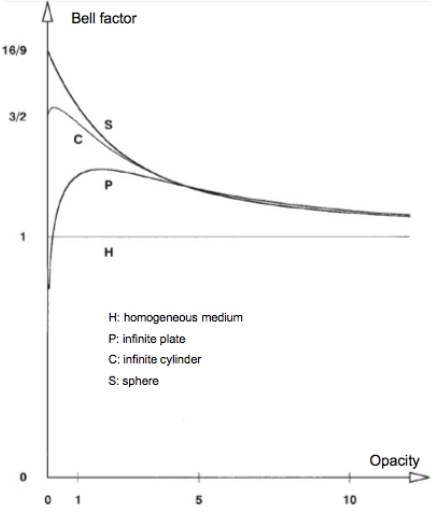
\includegraphics[width=3.5in]{images/r-m/bell.png}
  \caption{Bell's Factor for Various Geometris} \label{bell}
\end{figure}

[FIXME]: add materials from 2013 fall. We would typically compute a table of $P_{FF}$ as a function of opacity, and sample from it on the fly. 

Collision probability only gives us the average behavior in space and in energy. For instance, in CASMO when we run a 2D case we only have 8 energy groups. 

[FIXME] Lecture 9, p.6. An error in $P_{FF}$ leads to a bigger error in flux. Group flux is not very sensitive on the resonances (because the width of the resonances are small), so we need accurate group cross sections to capture the resonance behavior. 




\clearpage
\topic{Arrays of Rods, Dancoff Factor}
Notice our model so far is an isolated pin (that is, a fuel pin surrounded by an almost infinite moderator). Now we are going to discuss arrays of rods. The major difference is that not all neutrons leaving a fuel pin would have their next interaction in the moderator. 

We hence define the \hi{Dancoff Factor C}:
\eqn{ C = 1 - \frac{ \left. P_{f\to f} \right|_{\mbox{isolated rods}}}{ \left. P_{f\to f} \right|_{\mbox{arrays of rods}}}   }
In Fig.~\ref{dancoff}, the $x$-axis is the radius of the rods (in units of the mean free path of the moderators), and the curve also depends on the lattice size/radius of the rods (know that in a uniform square lattice, the lattice size is the pitch).  
\begin{figure}[ht]
  \centering
  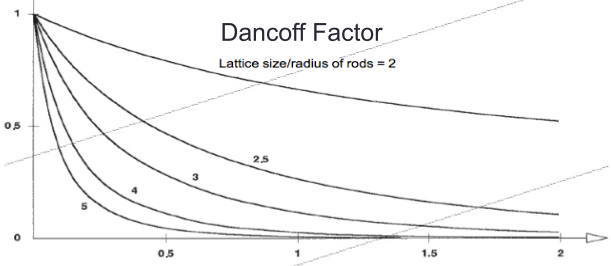
\includegraphics[width=4in]{images/r-m/dancoff.png}
  \caption{Dancoff Factor} \label{dancoff}
\end{figure}
\textbf{Notice if the moderator is opaque, the Dancoff factor becomes zero; if transparent, the Danoff factor trends to 1.0.}  LWRs typically have a C of 0.3. 
\eqn{ P_{f\to f}  = \frac{\sigma_{t,f} (u)}{\frac{(1-C)b}{(1-C) + Cb} \sigma_e + \sigma_{t,f} (u)}  } 
C changes the coefficient in front of the escape cross section from $\sigma_e \to \frac{(1-C)b}{1-C + Cb} \sigma_e$. For a typical PWR pin, that is reduced by 0.7 to 0.8.
\eqn{ \sigma_d &= \frac{D}{l N_0} + \frac{\Sigma_{fN}}{N_N} }
where $b = \frac{(1-C)b^+}{(1-C) + C b^+}$ where $b^+$ is the b factor for a single pin cell. 

\textbf{Example: Find Dancoff Factor.} Given water at 1 g/cc with a number density of $6.6 \times 10^{24}$ H atoms/cc, hydrogen xs of 20 barns, a PWR pin with 0.41 cm radius, a lattice pitch of 1.26cm. 
\begin{itemize}
\item We first find the mean free path: 
\eqn{ mfp = \frac{1}{\Sigma} = \frac{1}{N \sigma} =  \frac{1}{0.066 \times 10^{24} \times  20 \times 10^{-24}} =  0.76 \cm }
Then we find the parameter one, pellet radius over mfp = $\frac{0.41 \cm}{0.76 \cm}  = 0.54$, the other parameter is the lattice size over pellet radius $\frac{1.26 \cm}{0.41 \cm} = 3.07$. Using these two parameters, we can read off the plot that $C = 0.3$. For a Bell factor of about 1.1, the escape xs is reduced by,
\eqn{ \frac{ (1-C)b}{(1-C) + Cb} = 0.774} 
\end{itemize}
\hi{Remember 60 barns as the approximate average cross section for PWRs}. See slide 22 of Lecture 8. 






\clearpage
\topic{Carlvik's Refinements of the Bell's Collision Probability}
\eqn{ P_{ff} \approx \frac{\beta \sigma_{t,f}}{\alpha_1 + \sigma_e + \sigma_{t,f}} + \frac{(1-\beta) \sigma_{t,f}}{\alpha_2 \sigma_e + \sigma_{t,f}} }
where
\eqn{ \alpha_1 &= \frac{5A+6 - \sqrt{A^2 + 36A + 36}}{2(A+1)}, &\alpha_2 &= \frac{5A+6 + \sqrt{A^2 + 36A + 36}}{2(A+1)} &\beta&= \frac{\frac{4A+6}{A+1} - \alpha_1}{\alpha_2 - \alpha_1} &A&= \frac{1-C}{C} }
Carlvik's two-term approximation is what is actually used in production tools nowaday. To use it, we essentially look up the resonance integral (or group xs) twice, once with $\sigma_e$ multiplied by $\alpha_1$ and the second time with $\sigma_e$ multiplied by $\alpha_2$, each of them are simple functions of the Dancoff factor: 
\eqn{ \RIeff = \beta \int_{u1}^{u2} \sigma_r (u) \frac{\sigma_{pot, f} + \alpha_1 \sigma_e}{\sigma_{r,f}(u) + \sigma_{pot, f} + \alpha_1 \sigma_e} \du + (1-\beta) \int_{u1}^{u2} \sigma_r (u) \frac{\sigma_{pot,f} + \alpha_2 \sigma_e}{\sigma_{r,f}(u) + \sigma_{pot,f} + \alpha_2 \sigma_e} \du }
To double check, 
\begin{itemize}
\item $C\to 1, \alpha_1 \to 0, \beta \to 1$, e.g., there is no escape from fuel.
\item $C\to 0, \alpha_1 \to 2, \alpha_2 \to 3, \beta \to 2$, e.g., isolated rod.
\item For intermediate values of $C$, each coefficient is a monotonic function.
\end{itemize}
The beauty of this method is that the formula stays the same, we just have pre-tabulated table of the first and second terms depend on background xs. So given a background xs, we just need to table look-up the two terms and add them up. \\
\textbf{Recap}: moderator volume, cross section, density do matter when we come to arrys of rods through Dancoff factor.


\clearpage
\topic{Two-Region Pin Cell Code and Observations}
This section was covered in Lec10 of 22.211 (Spring 2012) and Lec 7 of 22.212 (Spring 2013). 
\begin{figure}[h]
  \centering
  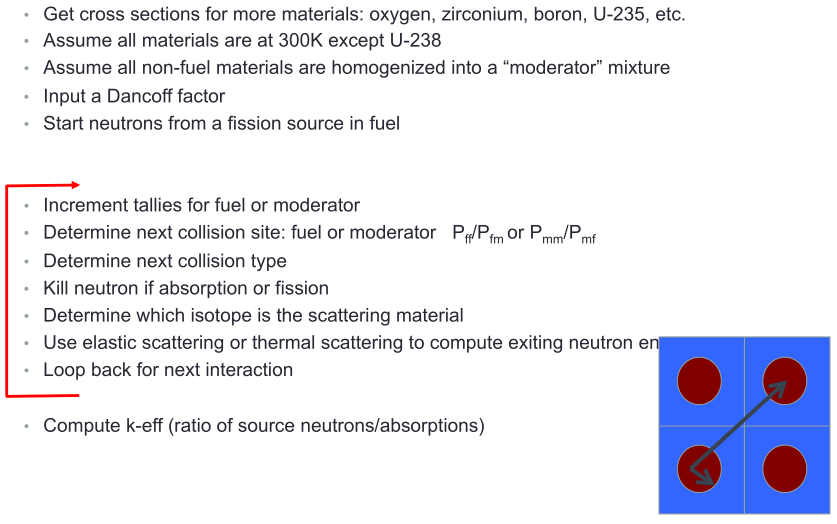
\includegraphics[width=4in]{images/r-m/pin-cell-code.png}
  \caption{Algorithm for a Simple Pin Cell Code with Collision Probabilities}
\end{figure}
\begin{enumerate}
\item With no oxygen or zirconium: flux dips in moderator are mild because there is only elastic scattering. See Fig.~\ref{pc-1}. 
\begin{figure}[h]
  \centering
  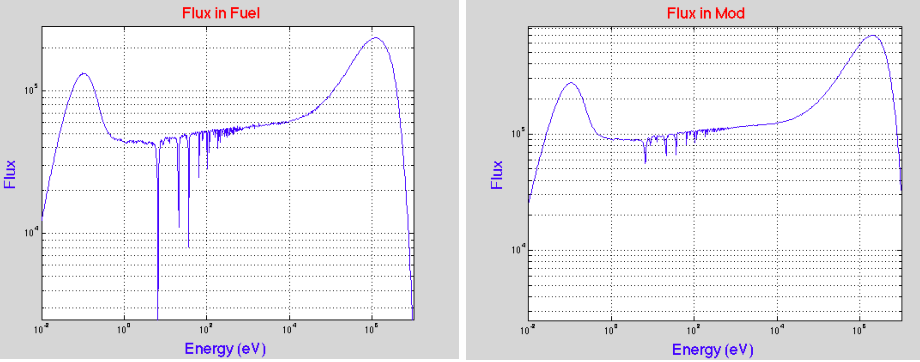
\includegraphics[width=4in]{images/r-m/pc-1.png}
  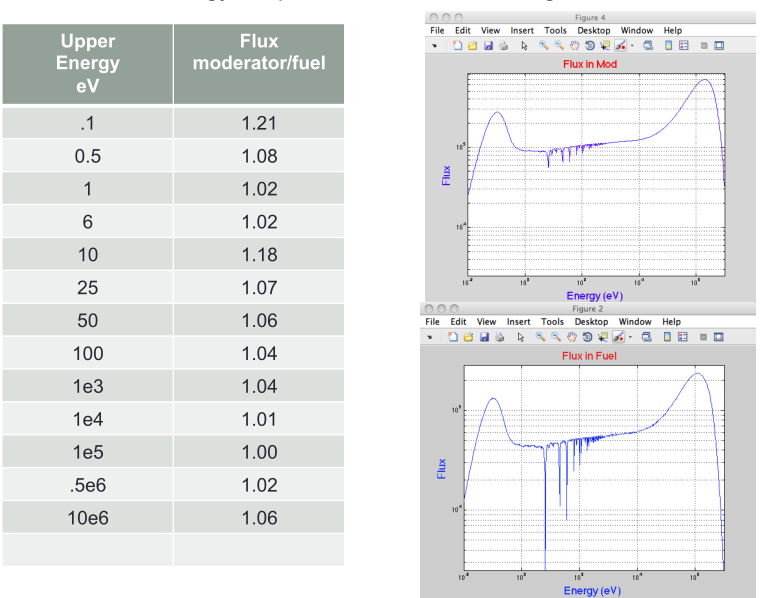
\includegraphics[width=4in]{images/r-m/pc-2.png}
  \caption{Pin Cell Code Results} \label{pc-1}
\end{figure}

\item Adding in Zr: Zr has massive elastic scattering resonances, hence creating fluctuations in both spectrums most noticable in energies right above the resonance energies. The reactivity change is small (positive 560 pcm). See Fig.~\ref{pc-3}. 
\begin{figure}[h]
  \centering
  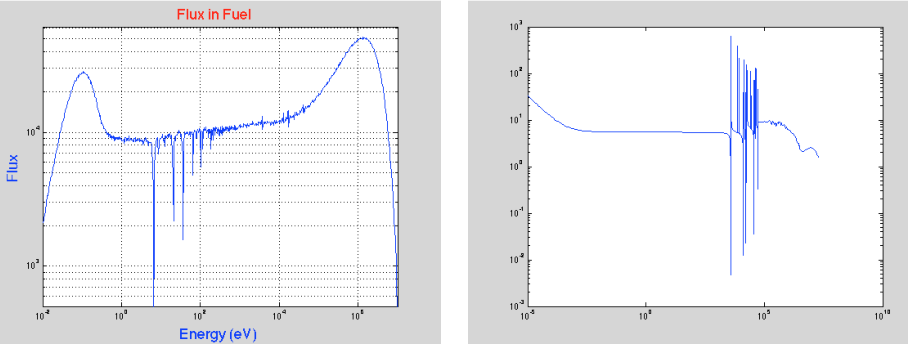
\includegraphics[width=4in]{images/r-m/pc-3.png}
  \caption{Pin Cell Code Results} \label{pc-3}
\end{figure}

\item Adding in O: the fast flux looks distorded in both fuel and moderator, this is because the oxygen xs has weird dips in high energy xs. The reactivity change is not large (negative 680 pcm).  See Fig.~\ref{pc-4}. 
\begin{figure}[h]
  \centering
  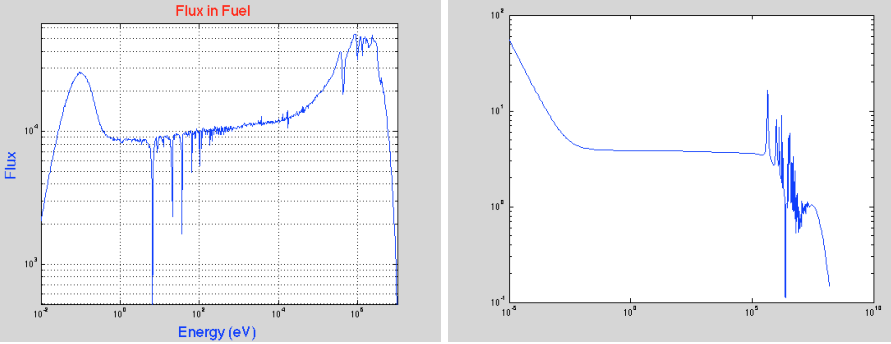
\includegraphics[width=4in]{images/r-m/pc-4.png}
  \caption{Pin Cell Code Results} \label{pc-4}
\end{figure}


\item Removing hydrogen absorption: the spectrum shape does not change much, but the reactivity change is huge (8808 pcm), because there are so much hydrogen, and that hydrogen xs is 1/v down to 100 keV. This is why LWR fuel has to be enriched. See Fig.~\ref{pc-5}. 
\begin{figure}[h]
  \centering
  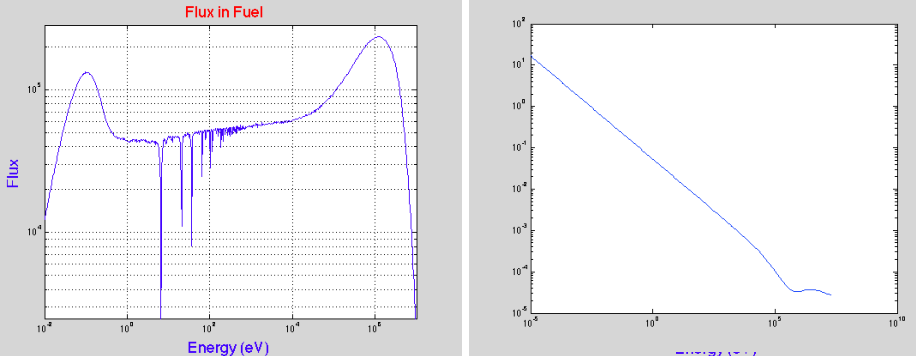
\includegraphics[width=4in]{images/r-m/pc-5.png}
  \caption{Pin Cell Code Results} \label{pc-5}
\end{figure}



\item Remove U238 fission: reduce reactivity by 2\% (negative -1910 pcm). Spectrum shape does not change. See Fig.~\ref{pc-6}. 
\begin{figure}[h]
  \centering
  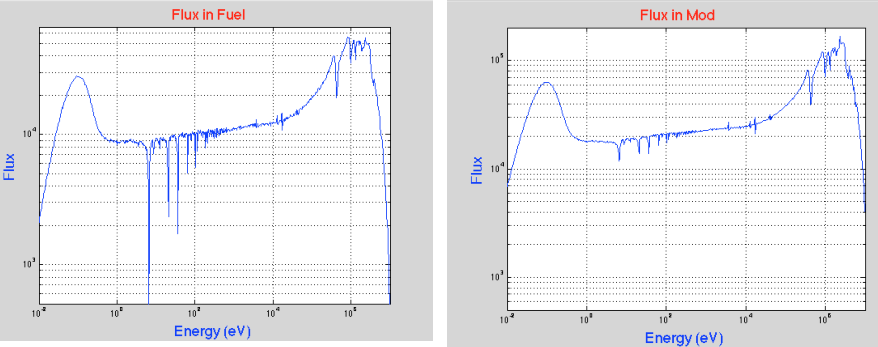
\includegraphics[width=4in]{images/r-m/pc-6.png}
  \caption{Pin Cell Code Results} \label{pc-6}
\end{figure}

\item PWR enrichment worth \hi{4.5\% $\Delta k$ per \%}. 

\item Doppler reactivity example: \hi{PWR Doppler worth = -2.7 pcm/K}. It is important to generate the Dopplar coefficient when preparing cross section data. 

\item Boron reactivity: Boron's capture cross section is almost entirely $(n,\alpha)$ cross section which produces He. \hi{Boron worth: $-16$ pcm/ppm}.
\end{enumerate}
Looking at the flux in the moderator divided by the flux in the fuel, we see that:
\begin{itemize}
\item Above resonance energies: fuel flux is depressed because absorption is high compared with fission; 
\item In resonance energies: larger than 1 because of fuel spectrums dips for the resonances; especially at the interval containing 6.7 eV;
\item Below resonance energies: the ratio is around 1, till we hit the really low energy (less than 0.1 eV), that there is a 1/E tail that the fuel flux gets depressed. 
\end{itemize}




\clearpage


\end{document}
